\documentclass[10pt,a4paper]{article}
\usepackage[utf8]{inputenc}
\usepackage{amsmath}
\usepackage{amsfonts}
\usepackage{amssymb}
\usepackage{graphicx}
\usepackage[left=1in,right=1in,top=1in,bottom=1in]{geometry}
\author{Ryan Honea}
\title{Unemployment Data Assessment}
\begin{document}
\maketitle
The US Unemployment Data given covers the range of January 1st, 1948 to March 1st, 2018. This means that it will include the sharp peaks in unemployment due to post war uncertainty, the aging of the baby boomers, and the various recessions in the 80s as well as the early 2000s. Because of this, there are high areas of uncertainty which lead to shying away from the classical ARMA model and utilizing a GARCH model for forecasting and analysis.

\begin{figure}[h]
\centering
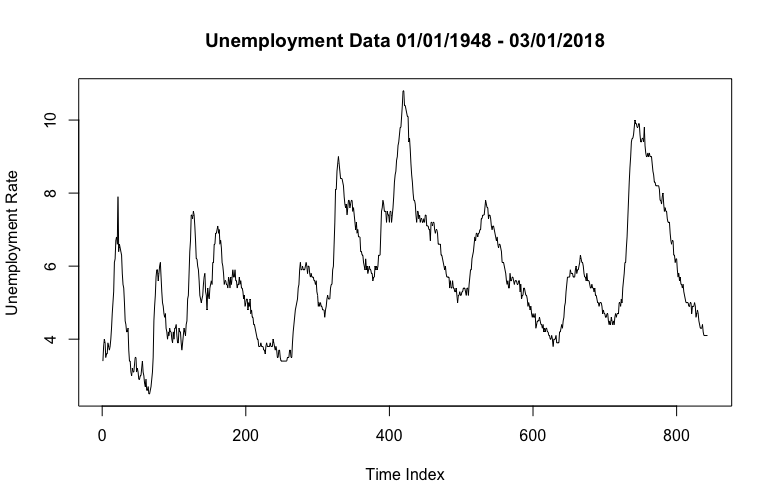
\includegraphics[scale=.5]{Dataplot}
\caption{Plot of Unemployment Data}
\end{figure}

Any model building of the data plotted in Figure 1 needs to account as well for the periods in which there is some degree of certainty, so the model utilized will be one that is mixed between the classical ARMA models as well as a GARCH model. First, we look at the Autocorellation Values for different lag values and then the Partial Autocorellation plots.

\begin{figure}[h]
\centering
\includegraphics[scale=.5]{TSDIsplay}
\caption{ACF and PACF Plots for Unemployment Data}
\end{figure}

Based on what we see in Figure 2, it appears that the data is purely or fractionally integrated. In order to confirm this, we utilize the Augment Dickey Fuller test to examine for stationarity.

\begin{verbatim}
	Augmented Dickey-Fuller Test

data:  x
Dickey-Fuller = -3.8912, Lag order = 9, p-value = 0.01444
alternative hypothesis: stationary
\end{verbatim}

These results suggest that the data is likely stationary under the alternate hypothesis, and thus does not necessarily have an integrated effect so we do not difference it. Some potential models then will consider the effects of the ARMA part of the process where the AR component has a strong effect on the MA component. We also account for the areas of high volatility by including a GARCH model thus giving us the following potential models:

\begin{itemize}
\item $ARMA(1,1) \times GARCH(1,1)$
\item $ARMA(1,1) \times GARCH(1,2)$
\item $ARMA(1,1) \times GARCH(2,1)$
\item $ARMA(1,1) \times GARCH(2,2)$
\end{itemize}

Most of these gave strong results, but the fourth model is chosen due to its strength and from it's residual diagnostics given in Figure 3.

\begin{figure}[h]
\centering
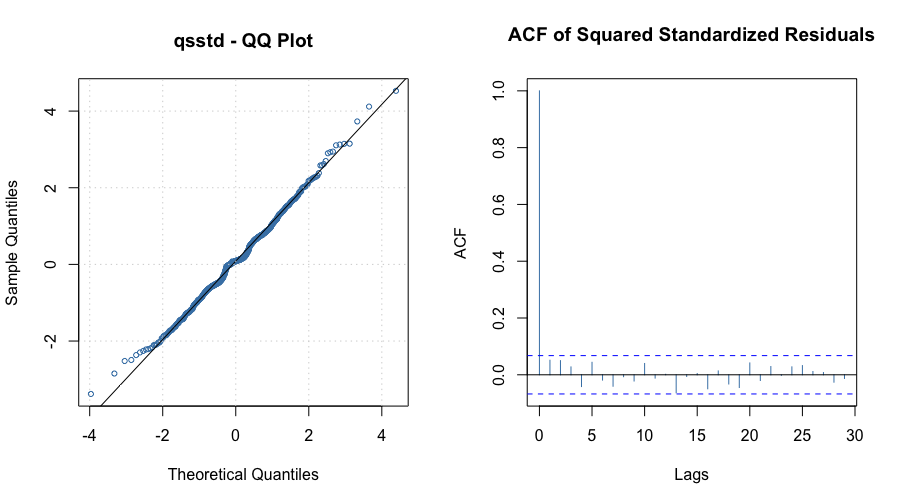
\includegraphics[width=.8\linewidth]{residualplots} 
\caption{ACF and PACF Plots for Unemployment Data}
\end{figure} 

The conditional distribution on the data is chosen to be the skewed standard t distribution due to the strength of its results. Additionally the Ljung-Box test on the squared values as well as the LM Arch test show that our residual values are not significantly different from our model.
\begin{verbatim}
 Ljung-Box Test     R^2  Q(10)  11.57381  0.3145912   
 Ljung-Box Test     R^2  Q(15)  15.1873   0.4380118   
 Ljung-Box Test     R^2  Q(20)  21.59956  0.3626288   
 LM Arch Test       R    TR^2   11.68884  0.4709819   
\end{verbatim}

The values of the coefficients are thus:
\begin{verbatim}
       mu        ar1        ma1      omega     alpha1     alpha2      beta1      beta2  
0.0439456  0.9890527  0.0129376  0.0033224  0.1479734  0.0846987  0.0973833  0.5863863  
     skew      shape  
1.0661094  8.4446449 
\end{verbatim}

When we forecast this data, we observe Figure 4 and see that the model determines that unemployment will stay roughly the same as its last point but will have high variance with increasing time as one might expect.

\begin{figure}[h]
\centering
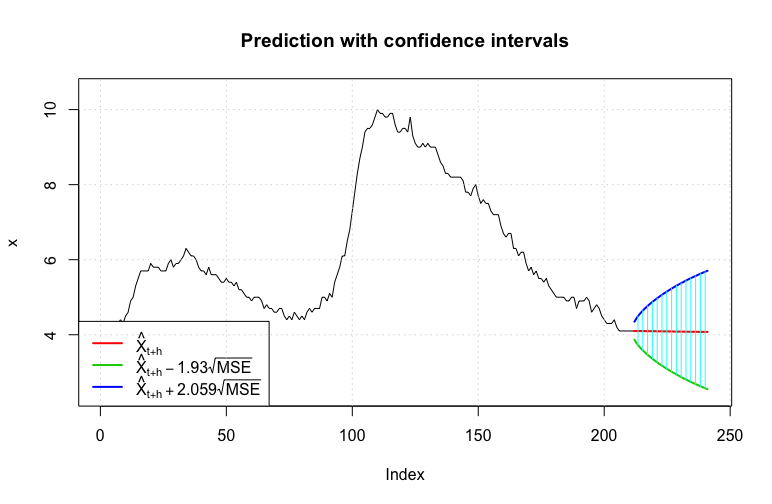
\includegraphics[scale=.5]{Forecast}
\caption{Forecast of Unemployment Data}
\end{figure}

\end{document}